Using the datasets from University of California Irvine Machine Learning Repository~\cite{uci_datasets}:

\begin{itemize}
\item White wine quality dataset~\cite{dataset_wine}, containing attributes and value like: fixed acidity,volatile acidity, citric acid and residual sugar,
\item Bike sharing dataset~\cite{dataset_bike_rental}, containing hourly and daily count of rental bikes between years 2011 and 2012 in Capital bikeshare system with the corresponding weather and seasonal information,
\item Steel plates faults dataset~\cite{dataset_steel_plates_faults}, describing faults of steel plates like, e.g.: scratches, depth of the scratch, bumps or height of bump.
\end{itemize}

While using the implemented solution with aforementioned datasets, parameter $k = 100$ has been chosen to gather the results.
Following graphs have been obtained:

\begin{figure}[h!]
  \centering
  \captionsetup{justification=centering}
    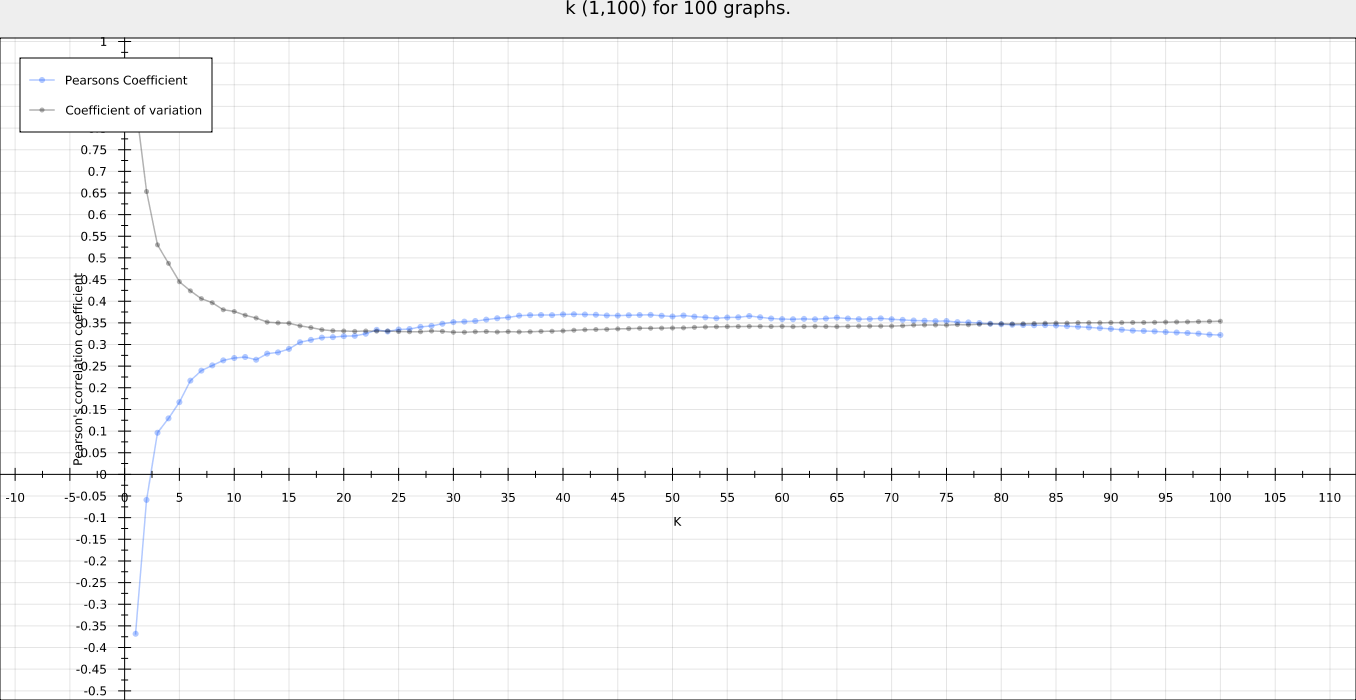
\includegraphics[width=1.05\textwidth]{images/k100_wine1000.png}
  \caption{Graph of Pearson correlation coefficient and its coefficient of variance against $K$ parameter for wine quality dataset.}
  \label{fig:graph_wine}
\end{figure}


\begin{figure}[h!]
  \centering
  \captionsetup{justification=centering}
    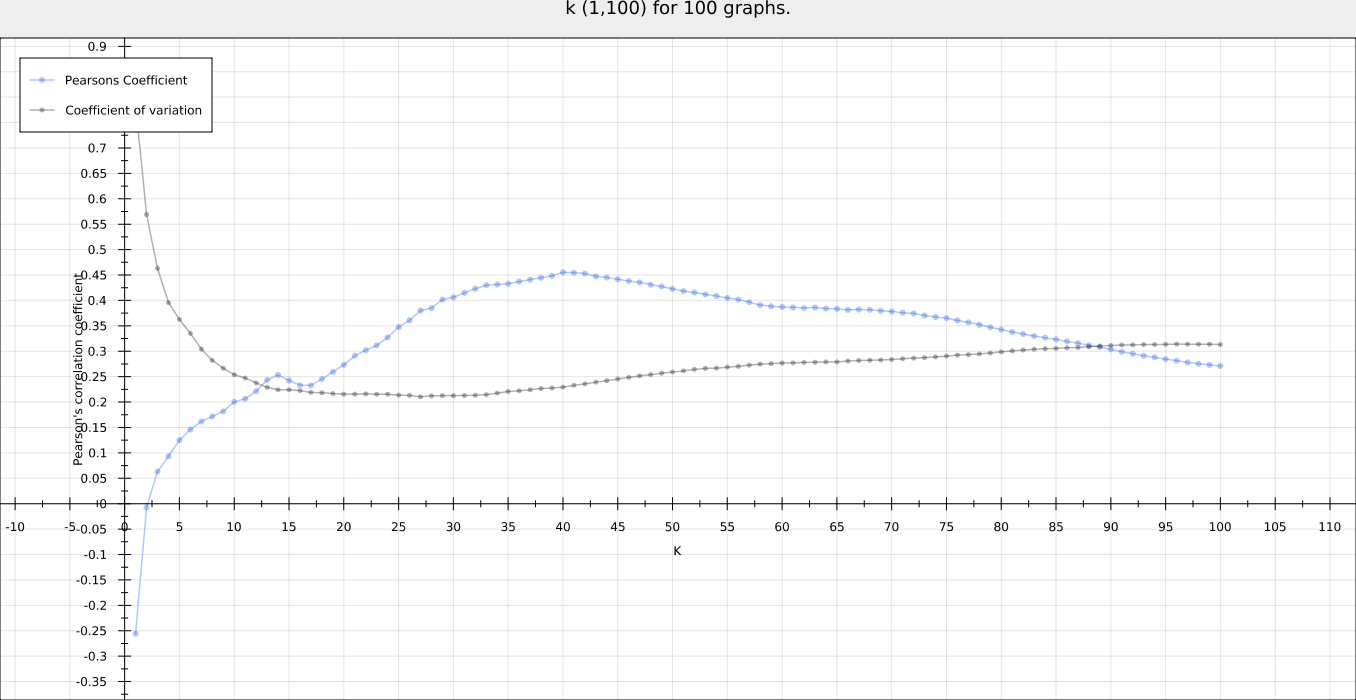
\includegraphics[width=1.05\textwidth]{images/k100_hour1000.png}
  \caption{Graph of Pearson correlation coefficient and its coefficient of variance against $K$ parameter for bike rental dataset.}
  \label{fig:graph_bike_rental}
\end{figure}


\begin{figure}[h!]
  \centering
  \captionsetup{justification=centering}
    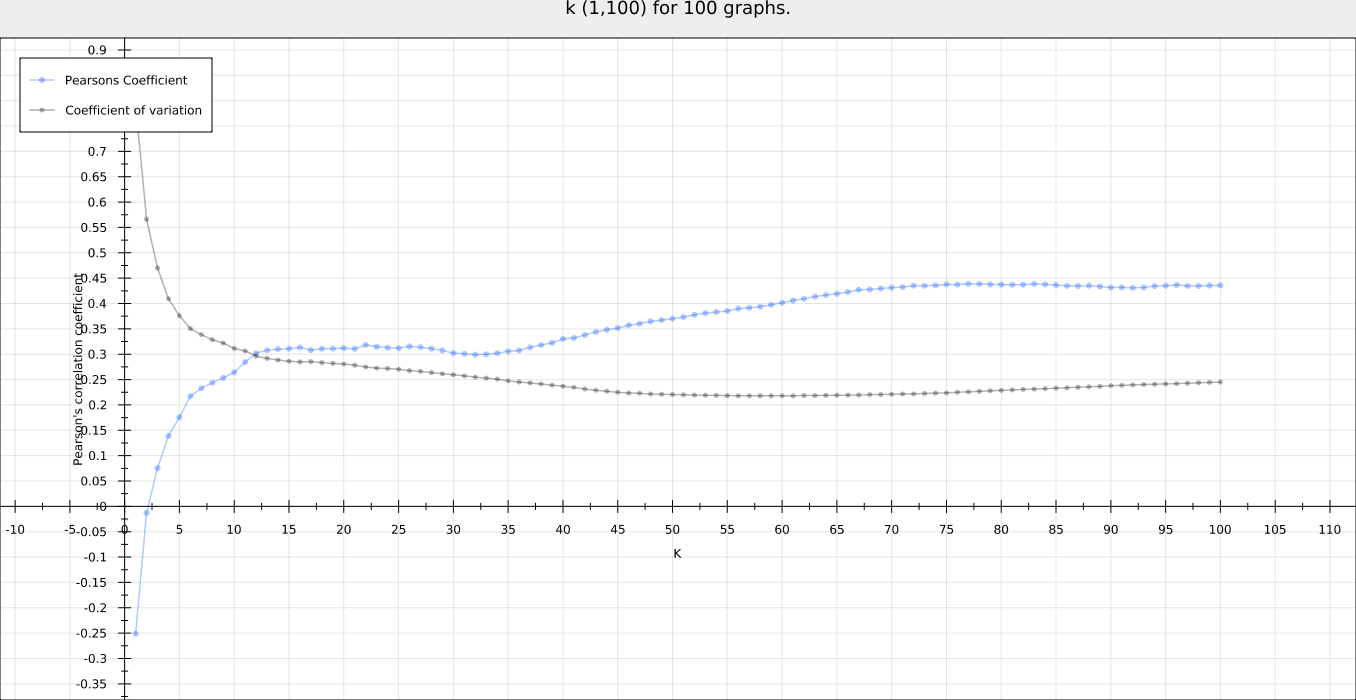
\includegraphics[width=1.05\textwidth]{images/k100_faults.png}
  \caption{Graph of Pearson correlation coefficient and its coefficient of variance against $K$ parameter for steel plates faults dataset.}
  \label{fig:graph_faults}
\end{figure}